% -----------------------------------------------------------------------------------------
% -----------------------------------------------------------------------------------------
% ---------- "A (very) short introduction to R" - Paul Torfs & Claudia Brauer -------------
% -----------------------------------------------------------------------------------------
% -----------------------------------------------------------------------------------------
% Current file is a modified version of the original TeX file, which was written by Paul
% Torfs & Claudia Brauer. It's the basic file for the greek translation of their respective
% introductory tutorial in R.
% -----------------------------------------------------------------------------------------
% -----------------------------------------------------------------------------------------

\documentclass[a4paper,11pt,twocolumn,tablecaptionabove]{scrartcl}

\usepackage{amssymb}
\bibliographystyle{plain}
\usepackage{multicol}
\usepackage{rotating}
\usepackage{url}
\usepackage{hyperref}
\usepackage{multirow}
\usepackage{a4wide}
\usepackage{graphicx}
\usepackage{wasysym}

% packages for R-intro chapter
\usepackage{pkg/fancybox}
\usepackage{pkg/fvrb-ex}

\usepackage[top=2.4cm, bottom=2.4cm, left=2cm, right=2cm]{geometry}
\setkomafont{captionlabel}{\bfseries} %% Bold float caption
\setcapindent{1em}

% -----------------------------------------------------------------------------------------
% Additional packages for greek language. -------------------------------------------------
\usepackage{fontspec}
\usepackage{xunicode}
\usepackage{xltxtra}
\usepackage{xgreek}
\setmainfont[Mapping=TeX-text]{Times New Roman}
% -----------------------------------------------------------------------------------------

% format of footnotes
\renewcommand{\thefootnote}{\fnsymbol{footnote}} % sets the footnotesymbols to fn in stead of numbers (already in use)
\deffootnote[1em]{0em}{1em}{\textsuperscript{\thefootnotemark}}

%%
%% The ToDo environment
%%
\usepackage[usenames,dvipsnames]{color}
 \newenvironment{ToDo} {%
  \begin{flushright}
    \hfill
    \begin{minipage}{0.95\columnwidth}         % used to be 0.95\columnwidth
    \textsf{\textbf{ToDo}} \\
      \vspace{-0.85cm}\\
      {\color{Gray}\rule[-0.1cm]{\columnwidth}{1.5pt}}} { % used to  be without 0.1cm
      {\color{Gray} \rule[0.3cm]{\columnwidth}{1.5pt}}
    \end{minipage}
    \vspace{1em}
  \end{flushright}
  }  
%%  

\makeatletter

\newcommand{\noun}[1]{\textsc{#1}}
%% Special footnote code from the package 'stblftnt.sty'
%% Author: Robin Fairbairns -- Last revised Dec 13 1996
\let\SF@@footnote\footnote
\def\footnote{\ifx\protect\@typeset@protect
 \expandafter\SF@@footnote
 \else
 \expandafter\SF@gobble@opt
 \fi
}
\expandafter\def\csname SF@gobble@opt \endcsname{\@ifnextchar[%]
 \SF@gobble@twobracket
 \@gobble
}
\edef\SF@gobble@opt{\noexpand\protect
 \expandafter\noexpand\csname SF@gobble@opt \endcsname}
\def\SF@gobble@twobracket[#1]#2{}

%%%%%%%%%%%%%%%%%%%%%%%%%%%%%%

\makeatother

% improve float handling
\renewcommand{\topfraction}{0.9}	
 \renewcommand{\bottomfraction}{0.8}	
 \setcounter{topnumber}{2}
 \setcounter{bottomnumber}{2}
 \setcounter{totalnumber}{4} 
 \setcounter{dbltopnumber}{2} 
 \renewcommand{\dbltopfraction}{0.9}	
 \renewcommand{\textfraction}{0.07}	
 \renewcommand{\floatpagefraction}{0.7}	
	% floatpagefraction MUST be less than topfraction !!
 \renewcommand{\dblfloatpagefraction}{0.7}

% change : to . in float caption
\renewcommand*{\captionformat}{\ } 

% package for making question boxes
\usepackage{boxedminipage}

% -----------------------------------------------------------------------------------------
% NOTES ON FORMATTING
% \texttt{...} is used to emphasize commands or clicking buttons in verbatim.
% \verb!...! is only used instead of \texttt{...} when there are brackets or other things
% \texttt can't handle.
% \emph is used to emphasize new terms
% -----------------------------------------------------------------------------------------

\title{\vspace{-13mm}A (very) short introduction to R}
\author{Paul Torfs \& Claudia Brauer\\
\footnotesize{Ομάδα Υδρολογίας και Ποσοτικής Διαχείρισης Υδάτων}\\
\footnotesize{Πανεπιστήμιο Wageningen, Ολλανδία}}
\date{\small{4 Νοεμβρίου 2014}}

\begin{document}

\maketitle

% -----------------------------------------------------------------------------------------
% [#01] Introduction
% -----------------------------------------------------------------------------------------
\section{Introduction}

Η R είναι μια ισχυρή γλώσσα και ένα ισχυρό περιβάλλον ανάπτυξης για στατιστικούς
υπολογισμούς και γραφικά. Ως έργο είναι κοινό κτήμα (ή αλλιώς είναι ένα λεγόμενο ``GNU" project),
το οποίο είναι παρόμοιο με την εμπορική γλώσσα και περιβάλλον S, που είχε αναπτυχθεί στα Bell 
Laboratories (πρώην AT\&T, πλέον Lucent Technologies) από τον John Chambers και τους συνεργάτες
του. Η R μπορεί να θεωρηθεί πως είναι μια διαφορετική υλοποίηση της S, και χρησιμοποιείται ευρέως
ως εκπαιδευτική γλώσσα και ερευνητικό εργαλείο.

Τα κύρια πλεονεκτήματα της R είναι το γεγονός ότι η R αποτελεί ελεύθερο λογισμικό και ότι υπάρχει
πολύ βοήθεια διαθέσιμη στο διαδίκτυο. Είναι αρκετά παρόμοια με άλλα προγραμματιστικά πακέτα όπως 
η MATLAB (που δεν είναι ελεύθερο λογισμικό), αλλά πιο φιλική προς τον χρήστη από γλώσσες
προγραμματισμού όπως η C++ και η Fortran. Μπορείτε να χρησιμοποιήσετε την R όπως είναι, αλλά για
εκπαιδευτικούς λόγους εμείς προτιμούμε τη χρήση της R σε συνδυασμό με την διεπαφή του RStudio (που είναι επίσης ελεύθερο λογισμικό), το οποίο έχει μια οργανωμένη διάταξη και διάφορες πρόσθετες
επιλογές.

Το παρόν έγγραφο περιλαμβάνει επεξηγήσεις, παραδείγματα και ασκήσεις, τα οποία (ελπίζουμε ότι)
μπορούν να γίνουν κατανοητά από ανθρώπους χωρίς καμία προγραμματιστική εμπειρία. Το διάβασμα
όλου του κειμένου και των ασκήσεων απαιτεί περίπου 1 με 2 ώρες. Παραδείγματα από εντολές που 
χρησιμοποιούνται συχνά και από μηνύματα λάθους παρατίθενται στις τελευταίες δύο σελίδες αυτού
του εγγράφου και μπορούν να χρησιμοποιηθούν ως αναφορά κατά τον προγραμματισμό.

% -----------------------------------------------------------------------------------------
% [#02] Getting started
% -----------------------------------------------------------------------------------------
\section{Getting started}

%%% [.01] -----------------------------------------------------------------------------------
\subsection{Install R}

Για να εγκαταστήσετε την R στον υπολογιστή σας (δωρεάν και με νόμιμο τρόπο!), πηγαίνετε στην
αρχική σελίδα του ιστοτόπου της R\footnote{Στον ιστότοπο της R μπορείτε επίσης να βρείτε και αυτό το παρόν έγγραφο: \url{http://cran.r-project.org/doc/contrib/Torfs+Brauer-Short-R-Intro.pdf}}:
\begin{quote}
  \url{http://www.r-project.org/}
\end{quote}
και εκτελέστε τα ακόλουθα (υποθέτοντας ότι δουλεύετε σε έναν υπολογιστή με Windows):\\
\noindent $\bullet$ κάντε κλικ στο \texttt{download CRAN} στην αριστερή στήλη\\
\noindent $\bullet$ επιλέξτε έναν ιστότοπο  για το download\\
\noindent $\bullet$ επιλέξτε \texttt{Windows} ως λειτουργικό σύστημα\\
\noindent $\bullet$ κάντε κλικ στο \texttt{base}\\
\noindent $\bullet$ επιλέξτε \texttt{Download R 3.0.3 for Windows} \footnote{Τη στιγμή της
συγγραφής του κειμένου αυτού η τελευταία έκδοση ήταν η 3.0.3. Επιλέξτε την πιο πρόσφατη.} και
αφήστε τις προεπιλεγμένες απαντήσεις σε όλες τις ερωτήσεις\\

Είναι επίσης πιθανό να εκτελέσετε την R και το RStudio από ένα USB αντί να τα εγκαταστήσετε. Αυτό
θα μπορούσε να είναι χρήσιμο όταν δεν έχετε δικαιώματα διαχειριστή στον υπολογιστή σας. Δείτε και 
την ξεχωριστή σημείωσή μας ``How to use portable versions of R and RStudio" για βοήθεια στο 
συγκεκριμένο θέμα.

%%% [.02] -----------------------------------------------------------------------------------
\subsection{Install RStudio}

Μετά την ολοκλήρωση της εγκατάστασης, θα πρέπει να βλέπετε ένα εικονίδιο "R" στην επιφάνεια
εργασίας σας. Κάνοντας κλικ σε αυτό θα εκκινήσετε την τυπική διεπαφή. Εμείς θα συνιστούσαμε,
ωστόσο, να χρησιμοποιήσετε την διεπαφή του RStudio. \footnote{Υπάρχουν πολλές άλλες διεπαφές
(ελεύθερου λογισμικού), όπως το Tinn-R.} Για να εγκαταστήσετε το RStudio, πηγαίνετε στον ιστότοπο: 
\begin{quote}
  \url{http://www.rstudio.org/}
\end{quote}
και εκτελέστε τα ακόλουθα (υποθέτοντας ότι δουλεύετε σε έναν υπολογιστή με Windows):\\
\noindent $\bullet$ κάντε κλικ στο \texttt{Download RStudio}\\
\noindent $\bullet$ κάντε κλικ στο \texttt{Download RStudio Desktop}\\
\noindent $\bullet$ κάντε κλικ στο \texttt{Recommended For Your System}\\
\noindent $\bullet$ κατεβάστε το \texttt{.exe} αρχείο και τρέξτε το 
(αφήστε τις προεπιλεγμένες απαντήσεις για όλες τις ερωτήσεις)

%%% [.03] -----------------------------------------------------------------------------------
\subsection{RStudio layout}

\begin{figure*}[htb]
  \centering
  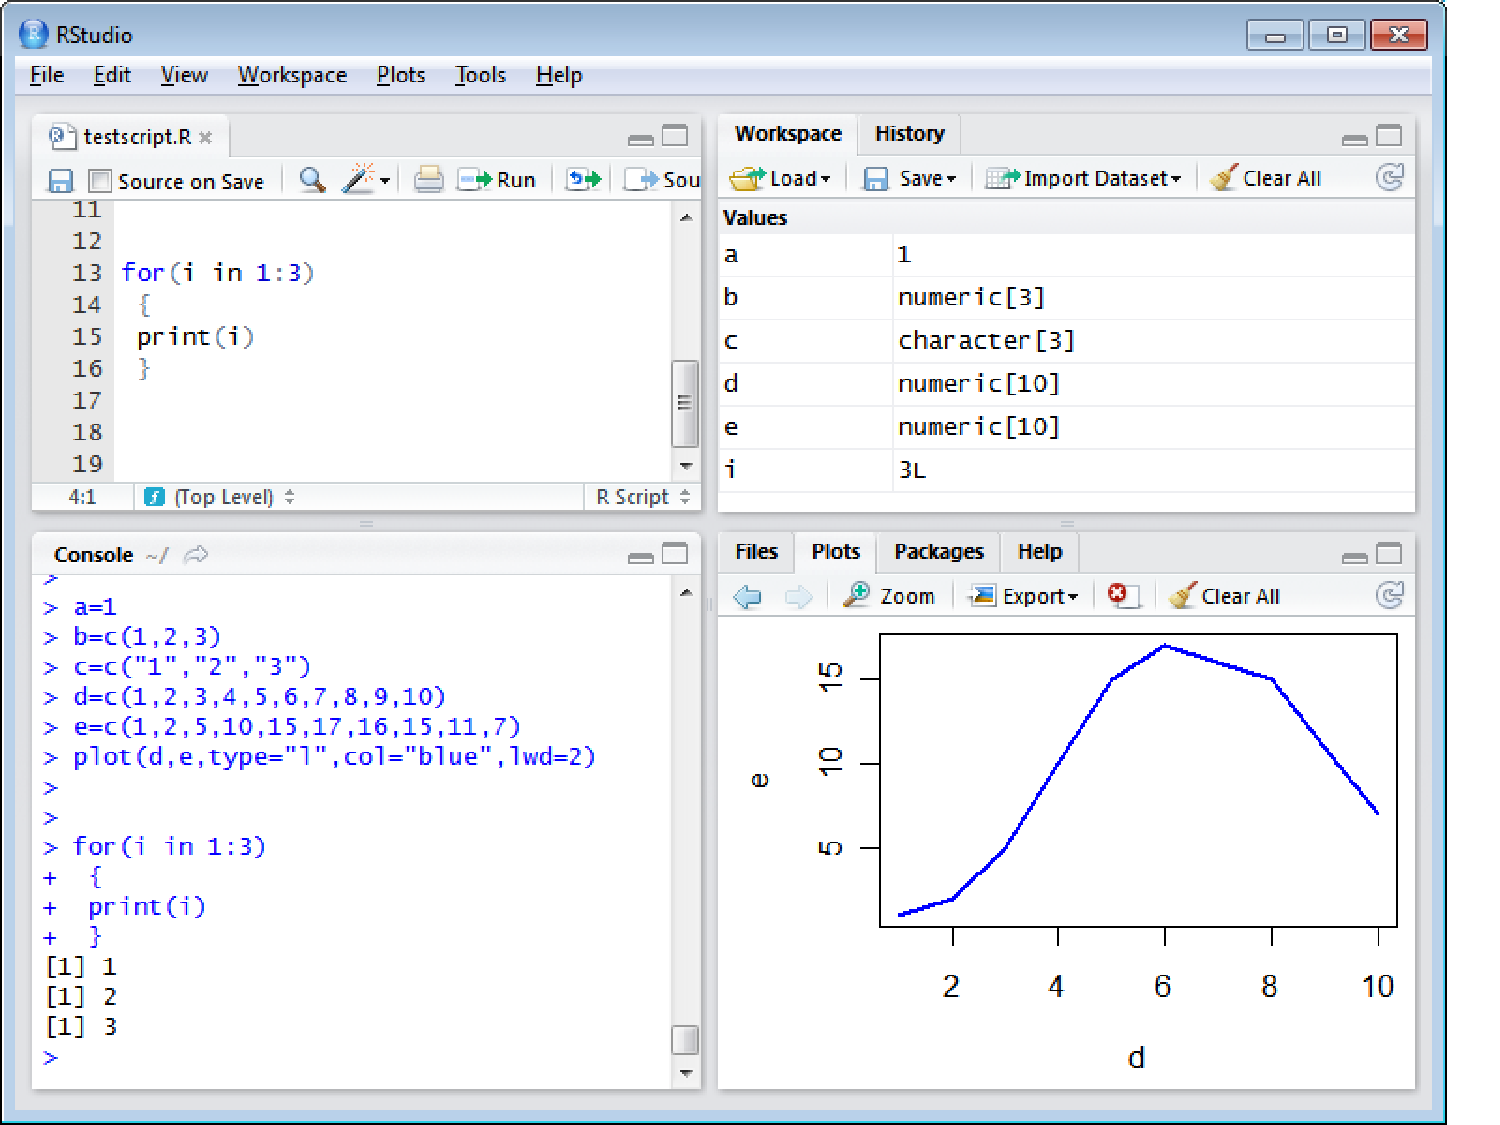
\includegraphics[width=13cm, clip=true, trim=0cm 0cm 9mm 0cm]{img/rstudio_screenshot.pdf}
  \caption{Τα παράθυρα του επεργαστή κειμένου, του χώρου εργασίας, της κονσόλας και των γραφικών παραστάσεων στο RStudio.}
  \label{fig:screenshot}
\end{figure*}

Η διεπαφή του RStudio αποτελείται από διάφορα παράδειγμα (βλέπε το Σχήμα~\ref{fig:screenshot}).
\begin{itemize}
\item Κάτω αριστερά: \textbf{παράθυρο κονσόλας} (που καλείται επίσης και \textbf{παράθυρο εντολών}). H
Εδώ μπορείτε να εισάγετε απλές εντολές μετά το σύμβολο υποβολής ``$>$'' και η R στη συνέχεια θα εκτελέσει
εντολή σας. Αυτό είναι το πιο σημαντικό παράθυρο, επειδή στην πραγματικότητα εκεί τρέχει η R.
\item Πάνω αριστερά: \textbf{παράθυρο επεξεργαστή κειμένου} (που καλείται επίσης και \textbf{παράθυρο σεναρίων}).
Εδώ μπορούν να υποστούν επεξεργασία και να σωθούν σύνολα από εντολές (σενάρια). Όταν δεν υπάρχει αυτό το
παράθυρο, μπορείτε να το ανοίξετε μέσω \texttt{File} $\rightarrow$ \texttt{New} $\rightarrow$ \texttt{R script}\\
Η απλή πληκτρολόγηση μιας εντολής στο παράθυρο του επεξεργαστή δεν είναι αρκετή, πρέπει επίσης να πάει και στο
παράθυρο εντολών πριν η R μπορέσει να εκτελέσει την εντολή αυτή. Εάν θέλετε να τρέξετε μία γραμμή από το 
παράθυρο σεναρίων (ή και ολόκληρο το σενάριο), μπορείτε να κάνετε κλικ στο \texttt{Run} ή να πατήσετε τα
πλήκτρα \texttt{CTRL+ENTER} ώστε να τη στείλετε στο παράθυρο εντολών. 
\item Πάνω δεξιά: \textbf{χώρος εργασίας / ιστορικό}. Στο παράθυρο του χώρου εργασίας
μπορείτε να δείτε ποια δεδομένα και ποιες τιμές έχει η R στη μνήμη της. Μπορείτε να δείτε και να επεξεργαστείτε
τις τιμές κάνοντας κλικ πάνω τους. Το παράθυρο του ιστορικού δείχνει το τι έχει πληκτρολογηθεί παλιότερα. 
\item Κάτω δεξιά: \textbf{αρχεία / γραφικές παραστάσεις / πακέτα / βοήθεια}. Από εδώ μπορείτε να ανοίξετε
αρχεία, να δείτε γραφικές παραστάσεις (και προηγούμενες γραφικές παραστάσεις, επίσης), να εγκαταστήσετε
και να φορτώσετε πακέτα ή να χρησιμοποιήσετε τη λειτουργία της βοήθειας.
\end{itemize}

Μπορείτε να αλλάξετε το μέγεθος των παραθύρων σέρνοντας τα γκρίζα διαχωριστικά μεταξύ των παραθύρων.

%%% [.04] -----------------------------------------------------------------------------------
\subsection{Working directory}

Ο \emph{κατάλογος εργασίας} σας είναι ο φάκελος του υπολογιστή σας μέσα στον οποίο εργάζεστε. Όταν ζητάτε από
την R να ανοίξει ένα συγκεκριμένο αρχείο, αυτή θα κοιτάξει πρώτα στον κατάλογο εργασίας γι' αυτό το αρχείο, και
όταν πείτε στην R να αποθηκεύσει ένα αρχείο δεδομένων ή ένα γράφημα, αυτή θα το αποθηκεύσει στον κατάλογο
εργασίας.

Πριν ξεκινήσετε να εργάζεστε, παρακαλούμε θέστε τον κατάλογο εργασίας σας εκεί που έχετε ή εκεί που πρέπει
να αποθηκεύονται όλα τα δεδομένα σας και τα αρχεία σεναρίων.

Εισάγετε στο παράθυρο εντολών το εξής: \verb!setwd("directoryname")!. Για παράδειγμα:
\begin{Verbatim}[frame=single,gobble=0]
> setwd("M:/Hydrology/R/")
\end{Verbatim}
Σιγουρευτείτε ότι οι μπάρες είναι πλάγιες μπάρες (/) και ότι δεν έχετε ξεχάσει τις αποστρόφους (για την ανάγκη
των αποστρόφων, δείτε στην ενότητα~\ref{sec:characters}). Η R διακρίνει τα πεζά από τα κεφαλαία γράμματα, οπότε
βεβαιωθείτε ότι γράφετε με κεφαλαία εκεί που απαιτείται.

Μέσα στο RStudio μπορείτε επίσης να πάτε στο \texttt{Tools / Set working directory}.

%%% [.05] -----------------------------------------------------------------------------------
\subsection{Libraries} 

Η R μπορεί να κάνει πολλές στατιστικές αναλύσεις και αναλύσεις δεδομένων. Αυτές είναι οργανωμένες στα 
λεγόμενα \emph{πακέτα} ή \emph{βιβλιοθήκες}. Με την τυπική εγκατάσταση, εγκαθίστανται και τα περισσότερα
συνήθη πακέτα. 

Για να δείτε μια λίστα με όλα τα εγκατεστημένα πακέτα, πηγαίνετε στο παράθυρο πακέτων ή πληκτρολογήστε 
\verb!library()! στο παράθυρο κονσόλας. Εάν το τετραγωνάκι μπροστά από το όνομα του πακέτου είναι τικαρισμένο,
το πακέτο φορτώνεται (ενεργοποιείται) και τότε μπορεί να χρησιμοποιηθεί. 

Υπάρχουν πολλά επιπλέον πακέτα διαθέσιμα στον ιστότοπο της R. Εάν θέλετε να εγκαταστήσετε και να χρησιμοποιήσετε
ένα πακέτο (για παράδειγμα, το πακέτο που λέγεται ``geometry"), τότε πρέπι να :\\
\noindent $\bullet$ Εγκαταστήσετε το πακέτο:  κάντε κλικ στο \texttt{install packages} στο παράθυρο πακέτων
και πληκτρολογήστε \texttt{geometry} ή εισάγετε την εντολή \verb!install.packages("geometry")! στο παράθυρο
εντολών.\\
\noindent $\bullet$ Φορτώστε το πακέτο: επιλέξτε το κουτάκι μπροστά από το \texttt{geometry} ή εισάγετε
την εντολή \verb!library("geometry")! στο παράθυρο εντολών.


% -----------------------------------------------------------------------------------------
% [#03] Some first examples of R commands
% -----------------------------------------------------------------------------------------
\section{Some first examples of R commands}

%%% [.01] -----------------------------------------------------------------------------------
\subsection{Calculator}

Η R μπορεί να χρησιμοποιηθεί ως αριθμομηχανή. Μπορείτε απλά να εισάγετε την εξίσωση που θέλετε στο
παράθυρο εντολών μετά από το ``$>$":
\begin{Verbatim}[frame=single,gobble=0]
> 10^2 + 36
\end{Verbatim}
and R will give the answer
\begin{Verbatim}[frame=single,gobble=0]
[1] 136
\end{Verbatim}

\begin{ToDo}
Υπολογίστε τη διαφορά μεταξύ του 2014 και του έτους στο οποίο ξεκινήσατε να σπουδάζετε σε αυτό το πανεπιστήμιο
και διαιρέστε το με τη διαφορά ανάμεσα στο 2014 και στο έτος το οποίο γεννηθήκατε. Πολλαπλασιάστε το επί 100 για
να πάρετε ως αποτέλεσμα το ποσοστό της ζωής σας που έχετε περάσει σε αυτό το πανεπιστήμιο. Χρησιμοποιήστε
παρενθέσεις, εάν χρειαστεί. \\
\end{ToDo}

Εάν χρησιμοποιήσετε παρενθέσεις και ξεχάσετε να προσθέσετε μια στο τέλος, το σύμβολο ``$>$" στη γραμμή
εντολών αλλάζει και γίνεται ``+". Το ``+" μπορεί επίσης να σημαίνει ότι η R είναι ακόμα απασχολημένη με 
κάποιον βαρύ υπολογισμό. Εάν θέλετε η R να σταματήσει αυτό που κάνει και να επανέλθει στο σύμβολο ``$>$", 
τότε πιέστε \texttt{ESC} (δείτε τη λίστα με τις αναφορές στην τελευταία σελίδα). 

%%% [.02] -----------------------------------------------------------------------------------
\subsection{Workspace}

Μπορείτε επίσης να δώσετε σε αριθμούς ένα όνομα. Κάνοντάς το αυτό, αυτοί μετατρέπονται στις λεγόμενες μεταβλητές,
οι οποίες μπορούν να χρησιμοποιηθούν αργότερα. Για παράδειγμα, μπορείτε να πληκτρολογήσετε στο παράθυρο εντολών
το εξής: 
\begin{Verbatim}[frame=single,gobble=0]
> a = 4
\end{Verbatim}
Μπορείτε να δείτε ότι το \texttt{a} εμφανίζεται στο παράθυρο του χώρου εργασίας, κάτι το οποίο σημαίνει ότι η
R πλέον θυμάται τι είναι το \texttt{a}.\footnote{Μερικοί προτιμούν τη χρήση του \texttt{<-} αντί του
\texttt{=} (κάνουν το ίδιο πράγμα). Το \texttt{<-} αποτελείται από δύο χαρακτήρες, τον \texttt{<} και τον
\texttt{-}, και συμβολίζει ένα βέλος που δείχνει στο αντικείμενο στο οποίο εκχωρείται η τιμή της έκφρασης.} 
Μπορείτε επίσης να ζητήσετε από την R να σας πει τι είναι το \texttt{a} (απλά πατήστε \texttt{a ENTER} στο
παράθυρο εντολών):

\begin{Verbatim}[frame=single,gobble=0]
> a 
[1] 4
\end{Verbatim}
or do calculations with \texttt{a}: 

\begin{Verbatim}[frame=single,gobble=0]
> a * 5
[1] 20
\end{Verbatim}

Εάν προσδιορίσετε ξανά το \texttt{a}, η R θα ξεχάσει τι τιμή είχε αυτό πριν. Μπορείτε επίσης να αναθέσετε μια
νέα τιμή στο \texttt{a} χρησιμοποιώντας την παλιά.

\begin{Verbatim}[frame=single,gobble=0]
> a = a + 10
> a
[1] 14
\end{Verbatim}

Για να απομακρύνετε όλες τις μεταβλητές από τη μνήμη της R, πληκτρολογήστε
\begin{Verbatim}[frame=single,gobble=0]
> rm(list=ls())
\end{Verbatim}
ή κάντε κλικ στο ``clear all" στο παράθυρο του χώρου εργασίας. Μπορείτε να δείτε ότι τότε το RStudio αδειάζει
το παράθυρο του χώρου εργασίας. Εάν θέλετε μόνο να απομακρύνετε τη μεταβλητή \texttt{a}, μπορείτε να πληκτρολογήσετε \texttt{rm(a)}.

\begin{ToDo}
Επαναλάβετε το προηγούμενο ToDo, αλλά με διάφορα βήματα ενδιάμεσα. Μπορείτε να δώστε στις μεταβλητές ό,τι όνομα
επιθυμείτε, αλλά κάθε όνομα πρέπει να ξεκινάει με ένα γράμμα. \\
\end{ToDo}

%%% [.03] -----------------------------------------------------------------------------------
\subsection{Scalars, vectors and matrices}

Όπως και πολλά άλλα προγράμματα, η R οργανώνει τους αριθμούς σε \emph{βαθμωτούς} (ένας απλός αριθμός --
μηδενικής διάστασης), σε \emph{διανύσματα} (μια ακολουθία αριθμών -- μονοδιάστατη) και σε \emph{μητρώα}
(όπως ένας πίνακας -- δισδιάστατα).

Το \texttt{a} που ορίσατε πριν ήταν ένας βαθμωτός. Για να ορίσετε ένα διάνυσμα με τους αριθμούς 3, 4 και 5,
χρειάζεστε τη συνάρτηση\footnote{Δείτε στην επόμενη ενότητα για την επεξήγηση των συναρτήσεων.} \texttt{c},
το όνομα της οποίας είναι το αρχικό του ρήματος concatenate (στα ελληνικά, συνενώνω). 
\begin{Verbatim}[frame=single,gobble=0]
b=c(3,4,5)
\end{Verbatim}

Τα μητρώα και οι υπόλοιπες δισδιάστατες δομές θα παρουσιαστούν στην ενότητα~\ref{sec:structures}.

%%% [.04] -----------------------------------------------------------------------------------
\subsection{Functions}

Εάν θέλετε να υπολογίσετε το μέσο όρο όλων των στοιχείων ενός διανύσματος \texttt{b} του παραπάνω παραδείγματος,
θα μπορούσατε να πληκτρολογήσετε 
\begin{Verbatim}[frame=single,gobble=0]
> (3+4+5)/3
\end{Verbatim}
Αλλά όταν το διάνυσμα είναι πολύ μεγάλο, αυτή η διαδικασία είναι πολύ βαρετή και χρονοβόρα. Γι' αυτό το λόγο
πράγματα τα οποία κάνετε συχνά αυτοματοποιούνται στις λεγόμενες \emph{συναρτήσεις}. Μερικές συναρτήσεις είναι 
εξαρχής στην R ή βρίσκονται σε κάποιο από τα πακέτα. Μπορείτε επίσης να προγραμματίσετε τις δικές σας 
συναρτήσεις (ενότητα~\ref{sec:progfunc}). Όταν θέλετε να χρησιμοποιήσετε μια συνάρτηση για να υπολογίσετε έναν
μέσο όρο, τότε θα πληκτρολογήσετε:
\begin{Verbatim}[frame=single,gobble=0]
> mean(x=b)
\end{Verbatim}

Μέσα στις παρενθέσεις προσδιορίζετε τα \emph{ορίσματα}. Τα ορίσματα παρέχουν επιπλέον πληροφορίες στη 
συνάρτηση. Στη συγκεκριμένη περίπτωση, το όρισμα \texttt{x} δηλώνει από ποιο σύνολο αριθμών (δηλαδή από ποιο
διάνυσμα) πρέπει να υπολογιστεί ο μέσος όρος (εδώ είναι του διανύσματος \texttt{b}). Μερικές φορές, το όνομα
του ορίσματος δεν είναι απαραίτητο: η εντολή \texttt{mean(b)} δουλεύει εξίσου καλά.

\begin{ToDo}
Υπολογίστε το άθροισμα των 4, 5, 8 και 11 αρχικά συνδυάζοντάς τα σε ένα διάνυσμα και έπειτα χρησιμοποιώντας
τη συνάρτηση \texttt{sum}.\\
\end{ToDo}

\begin{figure*}[htb]
  \centering
  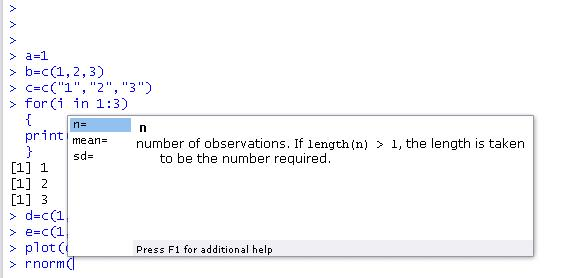
\includegraphics[width=10cm, clip=true, trim=0cm 0cm 0cm 1cm]{img/tab_RStudio.jpg}
  \caption{Το RStudio προτείνει πιθανά ορίσματα εάν πατήσετε το \texttt{TAB} μετά από το όνομα της συνάρτησης
  και την παρένθεση.}
  \label{fig:tab_RStudio}
\end{figure*}

Η συνάρτηση \texttt{rnorm}, πάλι για παράδειγμα, είναι μια πρότυπη συνάρτηση της R η οποία δημιουργεί
τυχαία δείγματα από μία κανονική κατανομή. Πιέστε το πλήκτρο \texttt{ENTER} και θα δείτε 10 τυχαίους αριθμούς
όπως οι ακόλουθοι:

\begin{Verbatim}[frame=single,numbers=left,gobble=0, xleftmargin=0.35cm, numbersep=0.1cm]
> rnorm(10)
[1] -0.949  1.342 -0.474 0.403 
[5] -0.091 -0.379  1.015  0.740 
[9] -0.639  0.950
\end{Verbatim}

\noindent $\bullet$ Η γραμμή 1 περιέχει την εντολή: η \texttt{rnorm} είναι η συνάρτηση και το 10 είναι το όρισμα
που ορίζει πόσους τυχαίους αριθμούς επιθυμείτε --- σε αυτήν την περίπτωση, 10 αριθμούς (πληκτρολογώντας
\texttt{n=10} αντί μόνο του \texttt{10} θα δούλευε επίσης).\\
\noindent $\bullet$ Οι γραμμές 2-4 περιέχουν τα αποτελέσματα: 10 τυχαίους αριθμούς τοποθετημένους σε ένα
διάνυσμα μήκους 10.

Η εισαγωγή της ίδιας εντολής ξανά παράγει 10 νέους τυχαίους αριθμούς. Αντί να πληκτρολογήσετε το ίδιο κείμενο 
πάλι, μπορείτε επίσης να πιέσετε το πλήκτρο με το άνω βελάκι ($\uparrow$) για να προσπελάσετε παλιότερες 
εντολές. Εάν θέλετε 10 τυχαίους αριθμούς από μία κανονική κατανομή με μέσο όρο 1.2 και τυπική απόκλιση 3.4,
μπορείτε να πληκτρολογήσετε
\begin{Verbatim}[frame=single,gobble=0]
> rnorm(10, mean=1.2, sd=3.4)
\end{Verbatim}
κάτι που δείχνει ότι η ίδια συνάρτηση (\texttt{rnorm}) μπορεί να έχει διαφορετικές διεπαφές και ότι η R έχει
τα λεγόμενα \emph{επώνυμα ορίσματα}  (σε αυτήν την περίπτωση τα \texttt{mean} και \texttt{sd}). Παρεπιπτόντως,
τα κενά γύρω από το ``," και το ``=" δεν μετράνε.

Συγκρίνοντας αυτό το παράδειγμα με το προηγούμενο βλέπει κανείς επίσης ότι για τη συνάρτηση \texttt{rnorm}
μόνο το πρώτο όρισμα (ο αριθμός 10) είναι υποχρεωτικό, και ότι η R δίνει προκαθορισμένες τιμές στα υπόλοιπα
προαιρετικά (όπως λέγονται) ορίσματα.\footnote{Χρησιμοποιήστε τη συνάρτηση help (ενότητα~\ref{sec:help}) για να
δείτε τις τιμές που χρησιμοποιούνται ως προκαθορισμένες.} 

Το RStudio έχει ένα ωραίο χαρακτηριστικό: εάν πληκτρολογήσετε \verb!rnorm(! στο παράθυρο εντολών και πιέσετε
\texttt{TAB}, τότε το RStudio θα εμφανίσει τα πιθανά ορίσματα (σχήμα~\ref{fig:tab_RStudio}).

%%% [.05] -----------------------------------------------------------------------------------
\subsection{Plots}

Η R μπορεί να φτιάξει γραφήματα. Το ακόλουθο είναι ένα πολύ απλό~\footnote{Δείτε την ενότητα
~\ref{sec:some-plotting} για λίγο λιγότερο «ασήμαντα» παραδείγματα.}
παράδειγμα:
\begin{Verbatim}[frame=single,numbers=left,gobble=0, xleftmargin=0.35cm, numbersep=0.1cm]
> x = rnorm(100)
> plot(x)
\end{Verbatim}

\noindent $\bullet$ Στην πρώτη γραμμή, εκχωρούνται 100 τυχαίοι αριθμοί στη μεταβλητή \texttt{x}, η οποία
γίνεται διάνυσμα μέσω αυτής της διαδικασίας. \\
\noindent $\bullet$ Στη δεύτερη γραμμή, όλες αυτές οι τιμές σχεδιάζονται στο παράθυρο γραφικών παραστάσεων.\\

\begin{ToDo}
Σχεδιάστε 100 τυχαίους (μέσω κανονικής κατανομής) αριθμούς.\\
\end{ToDo}


% -----------------------------------------------------------------------------------------
% [#04] Help and documentation
% -----------------------------------------------------------------------------------------
\section{Help and documentation}
\label{sec:help}

Υπάρχει διαθέσιμο πολύ υλικό από (δωρέαν) τεκμηρίωση και βοήθεια. Ένα μέρος της βοήθειας εγκαθίσταται
αυτόματα. Η πληκτρολόγηση στο παράθυρο της κονσόλας της εντολής
\begin{Verbatim}[frame=single,gobble=0]
> help(rnorm)
\end{Verbatim}
θα σας επιστρέψει βοήθεια πάνω στην συνάρτηση \texttt{rnorm}. Σας δίνει μια περιγραφή της συνάρτησης,
πιθανά ορίσματα και τις τιμές που χρησιμοποιούνται ως προεπιλογή για τα προαιρετικά ορίσματα. Εάν
πληκτρολογήσετε
\begin{Verbatim}[frame=single,gobble=0]
> example(rnorm)
\end{Verbatim}
θα σας επιστρέψει μερικά παραδείγματα του πώς μπορεί να χρησιμοποιηθεί αυτή η συνάρτηση.

Καθολική βοήθεια βασισμένη σε HTML μπορεί να κληθεί μέσω της εντολής:
An HTML-based global help can be called with:
\begin{Verbatim}[frame=single,gobble=0]
> help.start()
\end{Verbatim}
ή με τη μετάβαση στο παράθυρο βοήθειας.

Οι ακόλουθοι σύνδεσμοι μπορούν επίσης να φανούν πολύ χρήσιμοι:\\
\noindent $\bullet$ \url{http://cran.r-project.org/doc/manuals/ R-intro.pdf} Ένα πλήρες εγχειρίδιο.\\
\noindent $\bullet$ \url{http://cran.r-project.org/doc/contrib/ Short-refcard.pdf} Μια σύντομη καρτέλα
αναφοράς.\\
\noindent $\bullet$  \url{http://zoonek2.free.fr/UNIX/48\_R/all.html}\\
  Μια πολύ πλούσια πηγή παραδειγμάτων.\\
\noindent $\bullet$  \url{http://rwiki.sciviews.org/doku.php}\\
  Ένα τυπικό wiki για χρήστες.\\
\noindent $\bullet$ \url{http://www.statmethods.net/}\\
    Επίσης καλείται και Γρήγορη-R (Quick-R). Παρέχει πολύ παραγωγική και άμεση βοήθεια. Επίσης για χρήστες
    που έρχονται από άλλες γλώσσες προγραμματισμού. \\
    \noindent $\bullet$ \url{http://mathesaurus.sourceforge.net/}\\
    Λεξικό για γλώσσες προγραμματισμού (π.χ.~R για χρήστες Matlab). \\
\noindent $\bullet$  Και μόνο η χρήση της μηχανής Google (πληκτρολογήστε π.χ. ``R rnorm'' στο πεδίο αναζήτησης)
μπορεί να είναι πολύ παραγωγική.\\

\begin{ToDo}
Βρείτε βοήθεια για τη συνάρτηση \texttt{sqrt}.\\
\end{ToDo}


% -----------------------------------------------------------------------------------------
% [#05] Scripts
% -----------------------------------------------------------------------------------------
\section{Scripts}

Η R είναι ένας διερμηνέας που χρησιμοποιεί ένα περιβάλλον που βασίζεται στη γραμμή εντολών. Αυτό σημαίνει
ότι θα χρειάζεται να πληκτρολογείτε εντολές, αντί να χρησιμοποιείτε απλά το ποντίκι και τα μενού. Αυτό έχει
το πλεονέκτημα του ότι δε χρειάζεται εσείς να πληκτρολογείτε κάθε φορά ξανά όλες τις εντολές και έτσι έχετε
λιγότερες πιθανότητες να εμφανίσετε πόνους στα χέρια, το λαιμό και τους ώμους σας.

Μπορείτε να αποθηκεύετε τις εντολές σας σε αρχεία, τα λεγόμενα \emph{σενάρια}. Αυτά τα σενάρια έχουν τυπικά
ονόματα αρχείων με την κατάληξη \texttt{.R}, π.χ. \texttt{foo.R}. Μπορείτε να ανοίξετε τον επεξεργαστή κειμένου
σε ένα παράθυρο και να επεξεργαστείτε αυτά τα αρχεία κάνοντας κλικ στο \texttt{File} και \texttt{New} ή στο 
\texttt{Open file...}\footnote{Όπου είναι διαθέσιμες επίσης και οι επιλογές \texttt{Save} και
\texttt{Save as}.}.

Μπορείτε να τρέξετε (να στείλετε δηλαδή στο παράθυρο κονσόλας) ένα μέρος του κώδικα, επιλέγοντας γραμμές του και
πατώντας \texttt{CTRL+ENTER} ή κάνοντας κλικ στο \texttt{Run} στο παράθυρο του επεξεργαστή κειμένου. Εάν δεν
επιλέξετε κάτι, η R θα τρέξει τη γραμμή στην οποία βρίσκεται ο κέρσορας. Μπορείτε πάντα να τρέξετε όλο το
σενάριο με την εντολής κονσόλας \texttt{source}, κι έτσι π.χ. για το σενάριο στο αρχείο \texttt{foo.R} θα πρέπει
να πληκτρολογήσετε:
\begin{Verbatim}[frame=single,gobble=0]
> source("foo.R")
\end{Verbatim}
Μπορείτε επίσης να κάνετε κλικ στο \texttt{Run all} στο παράθυρο του επεξεργαστή κειμένου ή να
πατήσετε τα πλήκτρα \texttt{CTRL+SHIFT+S} ώστε να τρέξετε ολόκληρο το σενάριο με τη μία.

\begin{ToDo}
  Δημιουργήστε ένα αρχείο με όνομα \texttt{firstscript.R} το οποίο θα περιέχει κώδικα R που θα δημιουργεί 100
  τυχαίους αριθμούς και θα κάνει τη γραφική τους παράσταση, και τρέξτε αυτό το σενάριο αρκετές φορές.\\
\end{ToDo}


% -----------------------------------------------------------------------------------------
% [#06] Data structures
% -----------------------------------------------------------------------------------------
\section{Data structures} 
\label{sec:structures}

Εάν δεν είστε εξοικειωμένοι με την R, τότε είναι λογικό απλά να επαναπληκτρολογείτε τις εντολές που 
παρατίθενται σε αυτήν την ενότητα. Ίσως να μην χρειαστείτε όλες αυτές τις δομές στην αρχή, αλλά πάντα
είναι καλό να έχετε τουλάχιστον μια πρώτη εικόνα της ορολογίας και των πιθανών εφαρμογών.

%%% [.01] -----------------------------------------------------------------------------------
\subsection{Vectors}

Τα \emph{διανύσματα} τα έχουμε γνωρίσει ήδη, όμως μπορούν να κάνουν περισσότερα:

\begin{Verbatim}[frame=single,numbers=left,gobble=0, xleftmargin=0.35cm, numbersep=0.1cm]
> vec1 = c(1,4,6,8,10)
> vec1
[1]  1  4  6  8 10
> vec1[5]
[1] 10
> vec1[3] = 12
> vec1
[1]  1  4 12  8 10
> vec2 = seq(from=0, to=1, by=0.25)
> vec2
[1] 0.00 0.25 0.50 0.75 1.00
> sum(vec1)
[1] 35
> vec1 + vec2
[1]  1.00 4.25 12.50 8.75 11.00
\end{Verbatim}

\noindent $\bullet$  Στη γραμμή 1, ένα διάνυσμα \texttt{vec1} δημιουργείται ρητά από τη συνάρτηση συνένωσης
\texttt{c()}, την οποία έχουμε δει νωρίτερα. Τα στοιχεία των διανυσμάτων μπορούν να προσπελαστούν μέσω της
πρότυπης ευρετηρίασης \texttt{[i]}, όπως φαίνεται στις γραμμές 4-5. \\
\noindent $\bullet$  Στη γραμμή 6, ένα από τα στοιχεία αντικαθίσταται με ένα νέο αριθμό. Το αποτέλεσμα
εμφανίζεται στη γραμμή 8.\\
\noindent $\bullet$ Στη γραμμή 9 βλέπουμε ακόμα ένα χρήσιμο τρόπο δημιουργίας ενός διανύσματος: τη συνάρτηση
\texttt{seq()} (sequence ή ελληνιστί ακολουθία). \\
\noindent $\bullet$ Στις γραμμές 10-15 γίνονται μερικοί τυπικοί υπολογισμοί που αφορούν διανύσματα. Εάν
προσθέσετε δύο διανύσματα ίδιου μήκους, το πρώτο στοιχείο κάθε διανύσματος αθροίζεται με το άλλο, και το ίδιο
και το δεύτερο, κ.ο.κ., έχοντας ως αποτέλεσμα ένα νέο διάνυσμα μήκους 5 (ακριβώς όπως και στους κανονικούς
υπολογισμούς με διανύσματα). Προσέξτε ότι η συνάρτηση \texttt{sum} αθροίζει όλα τα στοιχεία ενός διανύσματος,
έχοντας ως αποτέλεσμα έναν αριθμό (ένα βαθμωτό).

%%% [.02] -----------------------------------------------------------------------------------
\subsection{Matrices}

Τα \emph{μητρώα} δεν είναι τίποτε άλλο παρά δισδιάστατα διανύσματα. Για να ορίσετε ένα μητρώο, χρησιμοποιήστε
τη συνάρτηση \texttt{matrix}:
\begin{Verbatim}[frame=single,numbers=left,gobble=0, xleftmargin=0.35cm, numbersep=0.1cm]
mat=matrix(data=c(9,2,3,4,5,6),ncol=3)
> mat
     [,1] [,2] [,3]
[1,]    9    3    5
[2,]    2    4    6
\end{Verbatim}

Το όρισμα \texttt{data} καθορίζει ποια νούμερα πρέπει να εισαχθούν στο μητρώο. Χρησιμοποιείστε είτε το 
\texttt{ncol} για να προσδιορίσετε τον αριθμό των στηλών είτε το \texttt{nrow} για να προσδιορίσετε τον
αριθμό των γραμμών. 

\begin{ToDo}
Εισάγετε τους αριθμούς από το 31 έως το 60 σε ένα διάνυσμα με όνομα \texttt{P} και σε ένα μητρώο με 6 γραμμές
και 5 στήλες με όνομα \texttt{Q}. Υπόδειξη: χρησιμοποιείστε τη συνάρτηση \texttt{seq}. Δείτε τους διάφορους
τρόπους με τους οποίους συμβολίζονται οι βαθμωτοί, τα διανύσματα και τα μητρώα στο παράθυρο του χώρου 
εργασίας.\\
\end{ToDo}
 
Οι πράξεις με μητρώα είναι παρόμοιες με τις πράξεις σε διανύσματα:

\begin{Verbatim}[frame=single,numbers=left,gobble=0, xleftmargin=0.35cm, numbersep=0.1cm]
> mat[1,2]
[1] 3
> mat[2,]
[1] 2 4 6
> mean(mat)
[1] 4.8333
\end{Verbatim}

\noindent $\bullet$ Τα στοιχεία ενός μητρώου μπορούν να προσπελαστούν με το συνήθη τρόπο: \texttt{[row,column]}
(γραμμή 1). \\
\noindent $\bullet$ Γραμμή 3: όταν θελήσετε να επιλέξετε μια ολόκληρη γραμμή, αφήστε τη θέση για το όρισμα του
αριθμού των στηλών κενή (και φυσικά το ανάποδο όταν θελήσετε στήλες).\\
\noindent $\bullet$ Στη γραμμή 5 βλέπουμε ότι πολλές συναρτήσεις εξακολουθούν να δουλεύουν όταν έχουν μητρώα
ως όρισμα.\\

%%% [.03] -----------------------------------------------------------------------------------
\subsection{Data frames}

Οι χρονοσειρές (time series) συχνά κατατάσσονται στα \emph{πλαίσια δεδομένων} (data frames). Ένα πλαίσιο
δεδομένων είναι ένα μητρώο με ονόματα πάνω από τις στήλες του. Αυτό είναι καλό, γιατί έτσι μπορείτε να καλέσετε
και να χρησιμοποιήσετε όποια από τις στήλες θέλετε χωρίς να γνωρίζετε σε ποια θέση είναι αυτή.
\begin{Verbatim}[frame=single,numbers=left,gobble=0, xleftmargin=0.35cm, numbersep=0.1cm]
> t = data.frame(x = c(11,12,14),
 y = c(19,20,21), z = c(10,9,7))
> t
   x y z
1 11 19 10
2 12 20 9 
3 14 21 7  
> mean(t$z)
[1] 8.666667
> mean(t[["z"]])
[1] 8.666667
\end{Verbatim}
%%$

\noindent $\bullet$ Στις γραμμές 1-2 κατασκευάζεται ένα τυπικό πλαίσιο δεδομένων με όνομα \texttt{t}. Οι στήλες
έχουν τα ονόματα \texttt{x}, \texttt{y} and \texttt{z}.\\
\noindent $\bullet$ Στις γραμμές 8-11 βλέπουμε δύο τρόπους με τους οποίους μπορείτε να επιλέξετε τη στήλη με 
όνομα \texttt{z} από το πλαίσιο δεδομένων με όνομα \texttt{t}.\\
\\

\begin{ToDo}
Δημιουργήστε ένα σενάριο το οποίο θα κατασκευάζει τρία τυχαία (κανονικά) διανύσματα μήκους 100. Ονομάστε
αυτά τα διανύσματα \texttt{x1}, \texttt{x2} και \texttt{x3}. Φτιάξτε ένα πλαίσιο δεδομένων με όνομα \texttt{t}
με τρεις στήλες (που θα λέγονται \texttt{a}, \texttt{b} και \texttt{c}) που θα περιέχει αντίστοιχα τα 
\texttt{x1}, \texttt{x1+x2} και \texttt{x1+x2+x3}. Καλέστε τις ακόλουθες συναρτήσεις για αυτό το πλαίσιο
δεδομένων: \texttt{plot(t)} και \texttt{sd(t\$x1)}. Μπορείτε να κατανοήσετε τα αποτελέσματα; Τρέξτε το
σενάριο ξανά μερικές φορές.\\
\end{ToDo}

%%% [.04] -----------------------------------------------------------------------------------
\subsection{Lists}

Μια άλλη βασική δομή στην R αποτελεί η \emph{λίστα}. Το κύριο πλεονέκτημα των λιστών είναι ότι οι «στήλες»
(δεν είναι πλέον διατεταγμένες σε στήλες, αλλά μοιάζουν πιο πολύ με μια συλλογή διανυσμάτων) δεν είναι
υποχρεωτικό να έχουν το ίδιο μήκος, αντίθετα με τις περιπτώσεις των μητρώων και των πλαισίων δεδομένων.

\begin{Verbatim}[frame=single,numbers=left,gobble=0, xleftmargin=0.35cm, numbersep=0.1cm]
> L = list(one=1, two=c(1,2), 
 five=seq(0, 1, length=5))
> L
$one
[1] 1
$two
[1] 1 2
$five
[1] 0.00 0.25 0.50 0.75 1.00
> names(L)
[1] "one"  "two"  "five"
> L$five + 10
[1] 10.00 10.25 10.50 10.75 11.00
\end{Verbatim}

\noindent $\bullet$ Στις γραμμές 1-2 δημιουργείται μια λίστα μέσω της εισόδου ονομάτων και τιμών. Η λίστα
εμφανίζεται επίσης και στο παράθυρο του χώρου εργασίας.\\
\noindent $\bullet$ Στις γραμμές 3-9 φαίνεται μια τυπική εκτύπωση (μετά από πάτημα των \texttt{L} και
\texttt{ENTER}). \\
\noindent $\bullet$ Η γραμμή 10 δείχνει πώς μπορούμε να δούμε τι υπάρχει μέσα στη λίστα.\\
\noindent $\bullet$ Η γραμμή 12 παρουσιάζει έναν τρόπο χρήσης των αριθμών. \\


% -----------------------------------------------------------------------------------------
% [#07] Graphics
% -----------------------------------------------------------------------------------------
\section{Graphics}
\label{sec:some-plotting}

Η σχεδίαση γραφικών παραστάσεων είναι μια σημαντική στατιστική δραστηριότητα. Οπότε δεν πρέπει να σας εκπλήσσει
το γεγονός ότι η R έχει πολλές δυνατότητες σχεδιασμού γραφικών παραστάσεων. Οι ακόλουθες γραμμές εμφανίζουν ένα
απλό γράφημα:
\begin{Verbatim}[frame=single,gobble=0]
> plot(rnorm(100), type="l", col="gold")
\end{Verbatim}

\noindent Εκατοντάδες τυχαίοι αριθμοί αναπαρίστανται γραφικά μέσω της σύνδεσης των σημείων με γραμμές (το 
σύμβολο μέσα σε εισαγωγικά μετά το \texttt{type=} είναι το γράμμα l, όχι ο αριθμός 1) σε χρυσό χρώμα.

Ένα άλλο πολύ απλό παράδειγμα είναι το κλασικό στατιστικό γράφημα του ιστογράμματος, που δημιουργείται από
την απλή εντολή
\begin{Verbatim}[frame=single,gobble=0]
  > hist(rnorm(100))
\end{Verbatim}
η οποία παράγει το γράφημα στο σχήμα~\ref{fig:hist}.
\begin{figure}[h]
  \centering
  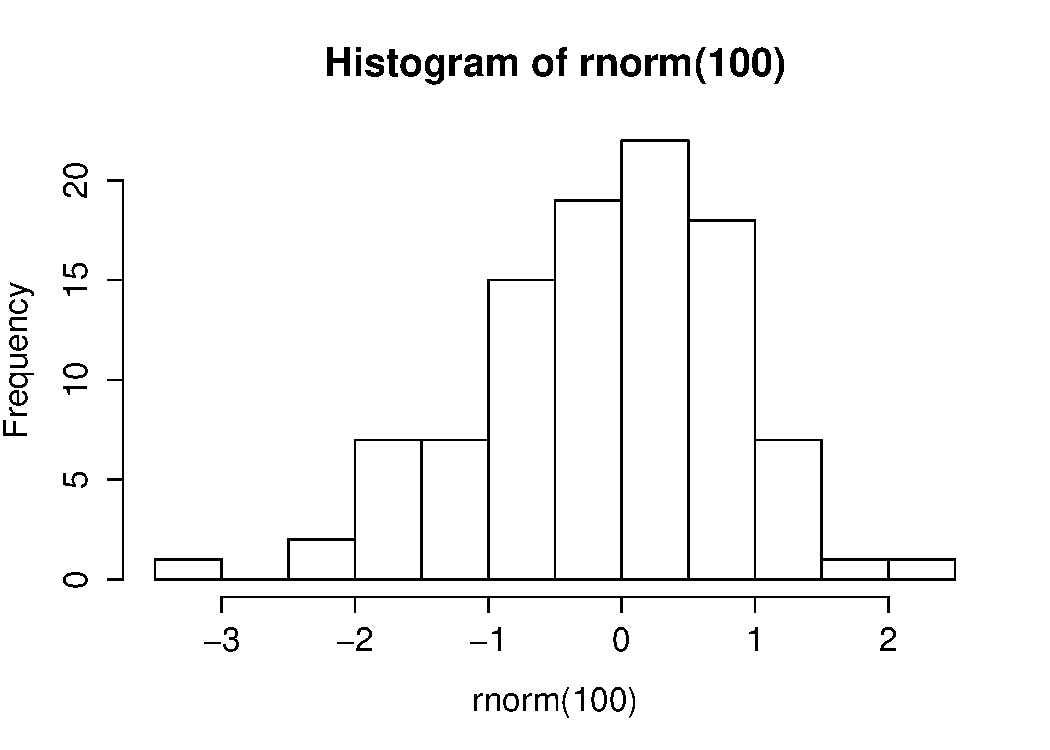
\includegraphics[width=8cm]{img/hist.pdf}
  \caption{Ένα απλό ιστόγραμμα.}
  \label{fig:hist}
\end{figure}

\noindent Οι ακόλουθες γραμμές δημιουργούν ένα γράφημα χρησιμοποιώντας το πλαίσιο δεδομένων \texttt{t} που 
φτιάξαμε στο προηγούμενο ToDo:
\begin{Verbatim}[frame=single,numbers=left,gobble=0, xleftmargin=0.35cm, numbersep=0.1cm]
plot(t$a, type="l", ylim=range(t), 
 lwd=3, col=rgb(1,0,0,0.3))
lines(t$b, type="s", lwd=2, 
 col=rgb(0.3,0.4,0.3,0.9))
points(t$c, pch=20, cex=4, 
 col=rgb(0,0,1,0.3))
\end{Verbatim} 
%%$ 

\begin{ToDo}
  Προσθέστε αυτές τις γραμμές στο αρχείο σεναρίου της προηγούμενης ενότητας. Δοκιμάστε να ανακαλύψετε, είτε 
  μέσω πειραματισμών, είτε με τη χρήση της βοήθειας, ποιο είναι το νόημα της \texttt{rgb}, του τελευταίου
  ορίσματος της \texttt{rgb}, του \texttt{lwd}, του \texttt{pch}, και του \texttt{cex}.\\
\end{ToDo}

Για να μάθετε περισσότερα σχετικά με τη μορφοποίηση των γραφημάτων, ψάξτε το \texttt{par} στη βοήθεια της R.
Κάντε αναζήτηση στη μηχανή της Google το ``R color chart" για να βρείτε ένα αρχείο pdf που περιέχει πλούτο
επιλογών χρωμάτων.

Για να αντιγράψετε τη γραφική σας παράσταση σε ένα έγγραφο, πηγαίνετε στο παράθυρο των γραφικών παραστάσεων,
κάντε κλικ στο κουμπί ``Export", επιλέξτε το μήκος και πλάτος που σας αρέσει περισσότερο και κάντε κλικ στο
\texttt{Copy} ή στο \texttt{Save}. 


% -----------------------------------------------------------------------------------------
% [#08] Reading and writing data files
% -----------------------------------------------------------------------------------------
\section{Reading and writing data files}
\label{sec:reading-writing-data}

Υπάρχουν πολλοί τρόποι για να καταγράψει κανείς δεδομένα σε αρχεία μέσω του περιβάλλοντος της R, και για να 
διαβάσει δεδομένα από αρχεία. Εδώ θα παρουσιάσουμε έναν τρόπο . Οι ακόλουθες γραμμές παρουσιάζουν τα στοιχειώδη:

\begin{Verbatim}[frame=single,numbers=left,gobble=0, xleftmargin=0.35cm, numbersep=0.1cm]
> d = data.frame(a = c(3,4,5), 
 b = c(12,43,54))
> d
  a  b
1 3 12
2 4 43
3 5 54
> write.table(d, file="tst0.txt",
 row.names=FALSE)
> d2 = read.table(file="tst0.txt", 
 header=TRUE)
> d2
  a  b
1 3 12
2 4 43
3 5 54
\end{Verbatim}
\noindent $\bullet$ Στις γραμμές 1-2, δημιουργείται ένα απλό πλαίσιο δεδομένων ως παράδειγμα και αποθηκεύεται 
στη μεταβλητή \texttt{d}. \\
\noindent $\bullet$ Στις γραμμές 3-7 φαίνεται το περιεχόμενο αυτού του πλαισίου δεδομένων: δύο στήλες (με 
όνομα \texttt{a} και \texttt{b}), κάθε μία από τις οποίες περιέχει τρεις αριθμούς.\\
\noindent $\bullet$ Στη γραμμή 8 καταγράφεται αυτό το πλαίσιο δεδομένων σε ένα αρχείο κειμένου, με όνομα
\texttt{tst0.txt} Το όρισμα \verb!row.names=FALSE! αποτρέπει τα ονόματα των γραμμών να καταγραφούν στο αρχείο.
Επειδή δεν καθορίζεται κάτι για τα \texttt{col.names}, επιλέγεται η προκαθορισμένη επιλογή \verb!col.names=TRUE!
και τα ονόματα των στηλών καταγράφονται στο αρχείο. Στο σχήμα~\ref{fig:tst0} φαίνεται το τελικό αρχείο 
(ανοιγμένο σε έναν επεξεργαστή κειμένου, όπως το Σημειωματάριο), με τα ονόματα των στηλών (\texttt{a} και
\texttt{b})στην πρώτη γραμμή. \\
\noindent $\bullet$ Οι γραμμές 10-11 δείχνουν πώς μπορούμε να εισάγουμε ένα αρχείο μέσα σε ένα πλαίσιο
δεδομένων. Σημειώστε ότι εισάγονται και τα ονόματα των στηλών. Το πλαίσιο δεδομένων εμφανίζεται επίσης στο
παράθυρο του χώρου εργασίας.\\

\begin{figure}[h]
  \centering
  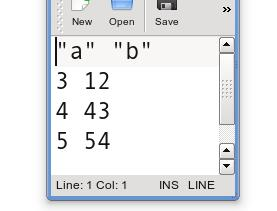
\includegraphics[width=3.5cm]{img/tst0.jpeg}
  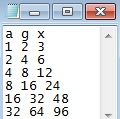
\includegraphics[width=2.6cm]{img/tst1.jpg}
  \caption{Τα αρχεία \texttt{tst0.txt} της ενότητας~\ref{sec:reading-writing-data}
    (αριστερά) και \texttt{tst1.txt} από το ToDo παρακάτω (δεξιά), ανοιγμένα σε δύο επεξεργαστές κειμένου.}
  \label{fig:tst0}
\end{figure}

\begin{ToDo}
  Φτιάξτε ένα αρχείο με όνομα \texttt{tst1.txt} στο Σημειωματάριο από το παράδειγμα του σχήματος~\ref{fig:tst0}
  και αποθηκεύστε το στον κατάλογο εργασίας σας. Γράψτε ένα σενάριο που να το διαβάζει, που να πολλαπλασιάζει
  τη στήλη με όνομα \texttt{g} επί 5 και να την αποθηκεύει με όνομα \texttt{tst2.txt}.\\
\end{ToDo}


% -----------------------------------------------------------------------------------------
% [#09] Not available data
% -----------------------------------------------------------------------------------------
\section{Not available data}

\begin{ToDo}
Υπολογίστε το μέσο όρο της τετραγωνικής ρίζας ενός διανύσματος 100 τυχαίων αριθμών. Τι θα συμβεί;
\end{ToDo}

Όταν δουλεύετε με πραγματικά δεδομένα, θα βρεθείτε αντιμέτωποι με τιμές που λείπουν επειδή υπήρξαν αστοχίες
στα όργανα μέτρηση ή επειδή δεν θέλατε να κάνετε μετρήσεις το Σαββατοκύριακο. Όταν ένα δεδομένο \emph{δεν
είναι διαθέσιμο}, τότε πρέπει να γράψετε \texttt{NA} αντί ενός αριθμού. 

\begin{Verbatim}[frame=single,gobble=0]
> j = c(1,2,NA)
\end{Verbatim}

Ο υπολογισμός στατιστικών από ημιτελή σύνολα δεδομένων είναι αδύνατος, αυστηρά μιλώντας. Μπορεί η μέγιστη τιμή
να εμφανίστηκε κατά τη διάρκεια του Σαββατοκύριακου, όταν δεν κάνατε μετρήσεις. Κατά συνέπεια, η R θα σας πει
ότι δε γνωρίζει ποια είναι η μέγιστη τιμή του \texttt{j}: 

\begin{Verbatim}[frame=single,gobble=0]
> max(j)
[1] NA
\end{Verbatim}

Εάν δεν έχετε πρόβλημα με τα δεδομένα που λείπουν και θέλετε να υπολογίσετε τα στατιστικά όπως και να 'χει,
μπορείτε να προσθέσετε το όρισμα \texttt{na.rm=TRUE} (να απομακρύνω/remove/rm τις τιμές NA; Ναι!). 

\begin{Verbatim}[frame=single,gobble=0]
> max(j, na.rm=TRUE)
[1] 2
\end{Verbatim}


% -----------------------------------------------------------------------------------------
% [#10] Classes
% -----------------------------------------------------------------------------------------
\section{Classes}

Οι ασκήσεις που κάνατε πριν ήταν σχεδόν όλες με αριθμούς. Μερικές φορές θα χρειαστεί να προσδιορίσετε κάτι το 
οποίο δεν είναι αριθμός, για παράδειγμα το όνομα ενός σταθμού μετρήσεων ή ενός αρχείο δεδομένων. Σε αυτήν την
περίπτωση θέλετε η μεταβλητή να είναι μια ακολουθία χαρακτήρων αντί για αριθμός. 

Ένα αντικείμενο στην R μπορεί να έχει διάφορες από τις λεγόμενες \emph{κλάσεις}. Οι τρεις πιο σημαντικές είναι
η \emph{numeric}, η \emph{character} και η \emph{POSIX} (συνδυασμοί ημερομηνίας-χρόνου). Μπορείτε να ρωτήσετε
την R ποια είναι η κλάση μιας συγκεκριμένης μεταβλητής πληκτρολογώντας \texttt{class(...)}. 

%%% [.01] -----------------------------------------------------------------------------------
\subsection{Characters}
\label{sec:characters}

Για να δηλώσετε στην R ότι κάτι είναι ακολουθία χαρακτήρων, πρέπει να πληκτρολογήσετε το κείμενο ανάμεσα από
αποστρόφους, αλλιώς η R θα αρχίσει να ψάχνει για μια καθορισμένη μεταβλητή με το ίδιο όνομα:

\begin{Verbatim}[frame=single,gobble=0]
> m = "apples"
> m
[1] "apples"
> n = pears
Error: object `pears' not found
\end{Verbatim}

Φυσικά, δεν μπορείτε να κάνετε υπολογισμούς με ακολουθίες χαρακτήρων:

\begin{Verbatim}[frame=single,gobble=0]
> m + 2
Error in m + 2 : non-numeric argument to 
binary operator
\end{Verbatim}

%%% [.02] -----------------------------------------------------------------------------------
\subsection{Dates}

Οι ημερομηνίες και οι χρόνοι είναι πολύπλοκοι. Η R πρέπει να να γνωρίζει ότι οι 3 η ώρα ακριβώς είναι μετά από
τις 2:59 και ότι ο Φεβρουάριος έχει 29 ημέρες σε μερικά έτη. Ο ευκολότερος τρόπος για να το πείτε στην R ότι κάτι αποτελεί συνδυασμό ημερομηνίας-ώρας είναι μέσω της συνάρτησης \texttt{strptime}:

\begin{Verbatim}[frame=single,numbers=left,gobble=0, xleftmargin=0.35cm, numbersep=0.1cm]
> date1=strptime( c("20100225230000", 
 "20100226000000", "20100226010000"), 
 format="%Y%m%d%H%M%S")
 > date1
[1] "2010-02-25 23:00:00" 
[2] "2010-02-26 00:00:00" 
[3] "2010-02-26 01:00:00"
\end{Verbatim}

\noindent $\bullet$  Στις γραμμές 1-2 δημιουργείτε ένα διάνυσμα με την \texttt{c(...)}. Οι αριθμοί στα 
διανύσματα είναι ανάμεσα σε αποστρόφους επειδή η συνάρτηση \texttt{strptime} απαιτεί ακολουθίες χαρακτήρων ως
είσοδο.\\
\noindent $\bullet$ Στη γραμμή 3 το όρισμα \texttt{format} προσδιορίζετι πώς θα πρέπει να διαβαστεί η ακολουθία
χαρακτήρων. Σε αυτή την περίπτωση το έτος αναπαρίσταται στην αρχή (\%Y), έπειτα ο μήνας (\%m), η ημέρα (\%d),
η ώρα (\%H), τα λεπτά (\%M) και τα δευτερόλεπτα (\%S). Δεν χρειάζεται να τα προσδιορίσετε όλα αυτά, εφόσον η
μορφή αυτή είναι αντίστοιχη με την ακολουθία εισόδου.

\begin{ToDo}
Δημιουργήστε ένα γράφημα, το οποίο θα έχει στον άξονα των x ημερομηνίες από τις 6 Δεκεμβρίου 2014 έως τα επόμενα 
γενέθλιά σας, και στον άξονα των y τον αριθμό των δώρων που περιμένετε σε κάθε μία από αυτές τις μέρες.
Υπόδειξη: φτιάξτε δύο διανύσματα πρώτα.
\end{ToDo}

% -----------------------------------------------------------------------------------------
% [#11] Programming tools
% -----------------------------------------------------------------------------------------
\section{Programming tools}

Όταν φτιάχνετε ένα μεγαλύτερο πρόγραμμα από τα προηγούμενα παραδείγματα ή όταν χρησιμοποιείτε τα σενάρια κάποιου
άλλου, μπορεί να συναντήσετε κάποιες προγραμματιστικές  δηλώσεις. Στην ενότητα αυτή θα περιγράψουμε μερικές
σχετικές συμβουλές και κόλπα.


%%% [.01] -----------------------------------------------------------------------------------
\subsection{If-statement}

Η δήλωση \emph{if} χρησιμοποιείται όταν συγκεκριμένοι υπολογισμοί πρέπει να γίνουν \emph{μόνο} όταν
ικανοποιείται μια συγκεκριμένη συνθήκη (και πιθανόν να πρέπει να γίνει κάτι άλλο όταν η συνθήκη δεν
ικανοποιείται). Ένα παράδειγμα:

\begin{Verbatim}[frame=single,numbers=left,gobble=0, xleftmargin=0.35cm, numbersep=0.1cm]
> w = 3
> if( w < 5 )
   {
   d=2
   }else{
   d=10
   }
> d
2
\end{Verbatim}

\noindent $\bullet$ Στη γραμμή 2 καθορίζεται μια συνθήκη: το \texttt{w} πρέπει να είναι μικρότερο του 5.\\
\noindent $\bullet$ Εάν η συνθήκη ικανοποιηθεί, τότε η R θα εκτελέσει ό,τι βρίσκεται ανάμεσα στις πρώτες αγκύλες
στη γραμμή 4.\\
\noindent $\bullet$ Εάν η συνθήκη \emph{δεν} ικανοποιηθεί, τότε η R θα εκτελέσει ό,τι βρίσκεται ανάμεσα στις
δεύτερες αγκύλες, μετά το \texttt{else} στης γραμμή 6. Μπορείτε να παραλείψετε το κομμάτι του \verb!else{...}!
εάν δεν το χρειάζεστε.\\
\noindent $\bullet$ Σε αυτή την περίπτωση, η συνθήκη ικανοποιείται και στη μεταβλητή \texttt{d} εκχωρείται
η τιμή 2 (γραμμές 8-9).

Για να πάρετε ένα υποσύνολο στοιχείων ενός διανύσματος για τα οποία ισχύει μια συγκεκριμένη συνθήκη, μπορείτε 
να χρησιμοποιήσετε μια πιο σύντομη μέθοδο:

\begin{Verbatim}[frame=single,numbers=left,gobble=0, xleftmargin=0.35cm, numbersep=0.1cm]
> a = c(1,2,3,4)
> b = c(5,6,7,8)
> f = a[b==5 | b==8]
> f
[1] 1 4
\end{Verbatim}

\noindent $\bullet$ Στη γραμμή 1 και 2 δημιουργούνται δύο διανύσματα.\\
\noindent $\bullet$ Στη γραμμή 3 δηλώνετε ότι η \texttt{f} συντίθεται από εκείνα τα στοιχεία του διανύσματος
\texttt{a} για τα οποία τα αντίστοιχα στοιχεία του \texttt{b} ισούται με 5 ή με 8. \\

Προσέξτε το διπλό \texttt{=} στη συνθήκη. Άλλες συνθήκες (που ονομάζονται επίσης λογικοί ή Boolean τελεστές)
είναι οι \texttt{<}, \texttt{>}, \texttt{!=} ($\neq$), \texttt{<=} ($\leq$) και \texttt{>=} ($\geq$). Για να
ελέγξετε περισσότερες από μία συνθήκες σε μία δήλωση if, χρησιμοποιήστε το \texttt{\&} εάν και οι δύο 
συνθήκες πρέπει να ικανοποιούνται (λογικό «και» - ``and") και το \texttt{|} εάν μία από τις συνθήκες πρέπει να 
ικανοποιείται (λογικό «ή» - ``or").

%%% [.02] -----------------------------------------------------------------------------------
\subsection{For-loop}

If you want to model a time series, you usually do the computations for one time step and then for the next and the next, etc. Because nobody wants to type the same commands over and over again, these computations are automated in for-loops. 

In a \emph{for-loop} you specify what has to be done and how many times. To tell ``how many times", you specify a so-called counter. An example:

\begin{Verbatim}[frame=single,numbers=left,gobble=0, xleftmargin=0.35cm, numbersep=0.1cm]
> h = seq(from=1, to=8)
> s = c()
> for(i in 2:10) 
   {
   s[i] = h[i] * 10
   }
> s
[1] NA 20 30 40 50 60 70 80 NA NA
\end{Verbatim}

\noindent $\bullet$ First the vector  \texttt{h} is made.\\
\noindent $\bullet$ In line 2 an empty vector ( \texttt{s}) is created. This is necessary because when you introduce a variable within the for-loop, R will not remember it when it has gotten out of the for-loop.\\
\noindent $\bullet$  In line 3 the for-loop starts. In this case, \texttt{i} is the counter and runs from 2 to 10.\\
\noindent $\bullet$ Everything between the curly brackets (line 5) is processed 9 times. The first time \texttt{i=2}, the second element of \texttt{h} is multiplied with 10 and placed in the second position of the vector \texttt{s}. The second time \texttt{i=3}, etc. In the last two runs, the 9$^\mathrm{th}$ and 10$^\mathrm{th}$ elements of \texttt{h} are requested, which do not exist. Note that these statements are evaluated without any explicit error messages.

\begin{ToDo}
Make a vector from 1 to 100. Make a for-loop which runs through the whole vector. Multiply the elements which are smaller than 5 and larger than 90 with 10 and the other elements with 0.1.
\end{ToDo}

%%% [.03] -----------------------------------------------------------------------------------
\subsection{Writing your own functions}
\label{sec:progfunc}

Functions you program yourself work in the same way as pre-programmed R functions.

\begin{Verbatim}[frame=single,numbers=left,gobble=0, xleftmargin=0.35cm, numbersep=0.1cm]
> fun1 = function(arg1, arg2 )
   {
   w = arg1 ^ 2
   return(arg2 + w)
   }
> fun1(arg1 = 3, arg2 = 5) 
[1] 14

\end{Verbatim}

\noindent $\bullet$ In line 1 the function name (\texttt{fun1}) and its arguments (\texttt{arg1} and \texttt{arg2}) are defined. \\
\noindent $\bullet$ Lines 2-5 specify what the function should do if it is called. The return value (\texttt{arg2+w}) is shown on the screen. \\
\noindent $\bullet$ In line 6 the function is called with arguments 3 and 5.

\begin{ToDo}
Write a function for the previous ToDo, so that you can feed it any vector you like (as argument). Use a for-loop in the function to do the computation with each element. Use the standard R function \texttt{length} in the specification of the counter. \footnote{Actually, people often use more for-loops than necessary. The ToDo above can be done more easily and quickly without a for-loop but with regular vector-computations.})
\end{ToDo}

\newpage


% -----------------------------------------------------------------------------------------
% [#12] Some useful references
% -----------------------------------------------------------------------------------------
\section{Some useful references}

%%% [.01] -----------------------------------------------------------------------------------
\subsection{Functions}

This is a subset of the functions explained in the R reference card.\\

\noindent \underline{Data creation}\\
$\bullet$ \texttt{read.table}: read a table from file. Arguments: \texttt{header=TRUE}: read first line as titles of the columns; \texttt{sep=","}: numbers are separated by commas; \texttt{skip=n}: don't read the first \texttt{n} lines.\\
$\bullet$ \texttt{write.table}: write a table to file\\
$\bullet$ \texttt{c}: paste numbers together to create a vector\\
$\bullet$ \texttt{array}: create a vector, Arguments: \texttt{dim}: length
$\bullet$ \texttt{matrix}: create a matrix, Arguments: \texttt{ncol} and/or \texttt{nrow}: number of rows/columns\\
$\bullet$ \texttt{data.frame}: create a data frame\\
$\bullet$ \texttt{list}: create a list\\
$\bullet$ \texttt{rbind} and \texttt{cbind}: combine vectors into a matrix by row or column\\

\noindent \underline{Extracting data}\\
$\bullet$ \texttt{x[n]}: the \texttt{n}$\mathrm{^{th}}$ element of a vector\\
$\bullet$ \texttt{x[m:n]}: the \texttt{m}$\mathrm{^{th}}$ to \texttt{n}$\mathrm{^{th}}$ element\\
$\bullet$ \texttt{x[c(k,m,n)]}: specific elements\\
$\bullet$ \texttt{x[x>m \& x<n]}: elements between \texttt{m} and \texttt{n}\\
$\bullet$ \verb!x$n!:  element of list or data frame named \texttt{n}\\  %$
$\bullet$ \texttt{x[["n"]]}: idem\\
$\bullet$ \texttt{[i,j]}: element at \texttt{i}$\mathrm{^{th}}$ row and\texttt{ }j$\mathrm{^{th}}$ column \\
$\bullet$ \texttt{[i,]}: row \texttt{i} in a matrix\\

\noindent \underline{Information on variables}\\
$\bullet$ \texttt{length}: length of a vector\\
$\bullet$ \texttt{ncol} or \texttt{nrow}: number of columns or rows in a matrix\\
$\bullet$ \texttt{class}: class of a variable \\
$\bullet$ \texttt{names}: names of objects in a list \\
$\bullet$ \texttt{print}: show variable or character string on the screen (used in scripts or for-loops) \\
$\bullet$ \texttt{return}: show variable on the screen (used in functions) \\
$\bullet$ \texttt{is.na}: test if variable is \texttt{NA}\\
$\bullet$ \texttt{as.numeric} or \texttt{as.character}: change class to number or character string\\
$\bullet$ \texttt{strptime}: change class from character to date-time (POSIX)\\

\noindent \underline{Statistics}\\
$\bullet$ \texttt{sum}: sum of a vector (or matrix)\\
$\bullet$ \texttt{mean}: mean of a vector\\
$\bullet$ \texttt{sd}: standard deviation of a vector\\
$\bullet$ \texttt{max} or \texttt{min}: largest or smallest element\\
%$\bullet$ \texttt{range}: min and max together\\
$\bullet$ \texttt{rowSums} (or \texttt{rowMeans}, \texttt{colSums} and \texttt{colMeans}): 
sums (or means) of all numbers in each row (or column) of a matrix. The result is a vector.\\
$\bullet$ \texttt{quantile(x,c(0.1,0.5))}: sample the 0.1 and 0.5$\mathrm{^{th}}$ quantiles of vector \texttt{x}\\

\noindent \underline{Data processing}\\
$\bullet$ \texttt{seq}: create a vector with equal steps between the numbers\\
$\bullet$ \texttt{rnorm}: create a vector with random numbers with normal distribution (other distributions are also available)\\
$\bullet$ \texttt{sort}: sort elements in increasing order\\
$\bullet$ \texttt{t}: transpose a matrix\\
$\bullet$ \texttt{aggregate(x,by=ls(y),FUN="mean")}: split data set \texttt{x} into subsets (defined by \texttt{y}) and computes means of the subsets. Result: a new list.\\
$\bullet$ \texttt{na.approx}: interpolate (in \texttt{zoo} package). Argument: vector with \texttt{NA}s. Result: vector without \texttt{NA}s.\\
$\bullet$ \texttt{cumsum}: cumulative sum. Result is a vector.\\
$\bullet$ \texttt{rollmean}: moving average (in the \texttt{zoo} package)\\
$\bullet$ \texttt{paste}: paste character strings together\\
$\bullet$ \texttt{substr}: extract part of a character string\\

\noindent \underline{Fitting}\\
$\bullet$ \texttt{lm(v1}$\thicksim$\texttt{v2)}: linear fit (regression line) between vector \texttt{v1} on the y-axis and \texttt{v2} on the x-axis\\
$\bullet$ \texttt{nls(v1}$\thicksim$\texttt{a+b*v2, start=ls(a=1,b=0))}: nonlinear fit. Should contain equation with variables (here \texttt{v1} and \texttt{v2} and parameters (here \texttt{a} and \texttt{b}) with starting values\\
$\bullet$ \texttt{coef}: returns coefficients from a fit\\
$\bullet$ \texttt{summary}: returns all results from a fit\\

\noindent \underline{Plotting}\\
$\bullet$ \texttt{plot(x)}: plot \texttt{x} (y-axis) versus index number (x-axis) in a new window\\
$\bullet$ \texttt{plot(x,y)}: plot \texttt{y} (y-axis) versus \texttt{x} (x-axis) in a new window\\
$\bullet$ \texttt{image(x,y,z)}: plot \texttt{z} (color scale) versus \texttt{x} (x-axis) and \texttt{y} (y-axis) in a new window\\
$\bullet$ \texttt{lines} or \texttt{points}: add lines or points to a previous plot \\
$\bullet$ \texttt{hist}: plot histogram of the numbers in a vector\\
$\bullet$ \texttt{barplot}: bar plot of vector or data frame\\
$\bullet$ \texttt{contour(x,y,z)}: contour plot\\
$\bullet$ \texttt{abline}: draw line (segment). Arguments: \texttt{a,b} for intercept \texttt{a} and slope \texttt{b}; or \texttt{h=y} for horizontal line at \texttt{y}; or \texttt{v=x} for vertical line at \texttt{x}. \\
$\bullet$ \texttt{curve}: add function to plot. Needs to have an \texttt{x} in the expression. Example: \verb!curve(x^2)! \\
$\bullet$ \texttt{legend}: add legend with given symbols (\texttt{lty} or \texttt{pch} and \texttt{col}) and text (\texttt{legend}) at location (\texttt{x="topright"})\\
$\bullet$ \texttt{axis}: add axis. Arguments: \texttt{side} -- \texttt{1}=bottom, \texttt{2}=left, \texttt{3}=top, \texttt{4}=right\\
$\bullet$ \texttt{mtext}: add text on axis. Arguments: \texttt{text} (character string) and \texttt{side}\\
$\bullet$ \texttt{grid}: add grid\\
$\bullet$ \texttt{par}: plotting parameters to be specified before the plots.  Arguments: e.g. \texttt{mfrow=c(1,3))}: number of figures per page (1 row, 3 columns); \texttt{new=TRUE}: draw plot over previous plot.\\

\noindent \underline{Plotting parameters}\\
These can be added as arguments to \texttt{plot}, \texttt{lines}, \texttt{image}, etc. For help see \texttt{par}.\\
$\bullet$ \texttt{type}: \texttt{"l"}=lines, \texttt{"p"}=points, etc.\\
$\bullet$ \texttt{col}: color -- \texttt{"blue"}, \texttt{"red"}, etc\\
$\bullet$ \texttt{lty}: line type -- \texttt{1}=solid, \texttt{2}=dashed, etc.\\
$\bullet$ \texttt{pch}: point type -- \texttt{1}=circle, \texttt{2}=triangle, etc.\\
$\bullet$ \texttt{main}: title - character string\\
$\bullet$ \texttt{xlab} and \texttt{ylab}: axis labels -- character string\\
$\bullet$ \texttt{xlim} and \texttt{ylim}: range of axes -- e.g. c(1,10)\\ 
$\bullet$ \texttt{log}: logarithmic axis -- \texttt{"x"}, \texttt{"y"} or \texttt{"xy"}\\

\noindent \underline{Programming}\\
$\bullet$ \verb!function(arglist){expr}!: function definition: do \texttt{expr} with list of arguments \texttt{arglist} \\ 
$\bullet$ \verb!if(cond){expr1}else{expr2}!: if-statement: if \texttt{cond} is true, then \texttt{expr1}, else \texttt{expr2} \\
$\bullet$ \verb!for(var in vec) {expr}!: for-loop: the counter \texttt{var} runs through the vector \texttt{vec} and does \texttt{expr} each run\\
$\bullet$ \verb!while(cond){expr}!: while-loop: while \texttt{cond} is true, do \texttt{expr} each run\\

%%% [.02] -----------------------------------------------------------------------------------
\subsection{Keyboard shortcuts}

There are several useful keyboard shortcuts for RStudio (see \texttt{Help} $\rightarrow$ \texttt{Keyboard Shortcuts}):\\
$\bullet$ \texttt{CRL+ENTER}: send commands from script window to command window\\
$\bullet$ $\uparrow$ or $\downarrow$ in command window: previous or next command\\
$\bullet$ \texttt{CTRL+1}, \texttt{CTRL+2}, etc.: change between the windows\\

\noindent Not R-specific, but very useful keyboard shortcuts:\\
$\bullet$ \texttt{CTRL+C}, \texttt{CTRL+X} and \texttt{CTRL+V}: copy, cut and paste\\
$\bullet$ \texttt{ALT+TAB}: change to another program window\\
$\bullet$ $\uparrow$, $\downarrow$, $\leftarrow$ or $\rightarrow$: move cursor\\
$\bullet$ \texttt{HOME} or \texttt{END}: move cursor to begin or end of line\\
$\bullet$ \texttt{Page Up} or \texttt{Page Down}: move cursor one page up or down\\
$\bullet$ \texttt{SHIFT+$\uparrow$/$\downarrow$/$\leftarrow$/$\rightarrow$/HOME/END/PgUp/PgDn}: select\\

%%% [.03] -----------------------------------------------------------------------------------
\subsection{Error messages}

\noindent $\bullet$ \texttt{No such file or directory} or \texttt{Cannot change working directory} \\
Make sure the working directory and file names are correct.\\
\noindent $\bullet$ \texttt{Object `x' not found}\\
The variable \texttt{x} has not been defined yet. Define \texttt{x} or write apostrophes if \texttt{x} should be a character string.\\
\noindent $\bullet$ \texttt{Argument `x' is missing without default}\\
You didn't specify the compulsory argument \texttt{x}.\\
\noindent $\bullet$ \texttt{+}\\ %
R is still busy with something or you forgot closing brackets. Wait, type \verb!}! or \verb!)! or press \texttt{ESC}.\\ %
\noindent $\bullet$ \verb!Unexpected ')' in ")"! or \verb!Unexpected '}'! \verb!in "}"!\\ 
The opposite of the previous. You try to close something which hasn't been opened yet. Add opening brackets.\\
\noindent $\bullet$ \texttt{Unexpected `else' in "else"}\\
Put the \verb!else! of an if-statement on the same line as the last bracket of the ``then"-part: \verb!}else{!.\\
\noindent $\bullet$ \texttt{Missing value where TRUE/FALSE needed}\\
Something goes wrong in the condition-part (\texttt{if(x==1)}) of an if-statement. Is \texttt{x} \texttt{NA}? \\
\noindent $\bullet$ \texttt{The condition has length > 1 and only the first element will be used}\\
In the condition-part (\texttt{if(x==1)}) of an if-statement, a vector is compared with a scalar. Is \texttt{x} a vector? Did you mean \texttt{x[i]}?\\
\noindent $\bullet$ \texttt{Non-numeric argument to binary operator} \\
You are trying to do computations with something which is not a number. Use \texttt{class(...)} to find out what went wrong or use \texttt{as.numeric(...)} to transform the variable to a number.\\
\noindent $\bullet$ \texttt{Argument is of length zero} or \texttt{Replacement is of length zero}\\
The variable in question is \texttt{NULL}, which means that it is empty, for example created by \texttt{c()}. Check the definition of the variable.
%\noindent $\bullet$ \texttt{Subscript out of bounds}\\
%You are asking for an element of vector or matrix which doesn't exist (\texttt{x[4]} when \texttt{x} is just 3 elements long. This often happens when a for-loop starts too early or late.\\

%\noindent $\bullet$ \verb!Object of type 'closure' is not subset-! \verb!table!\\
%Something goes wrong when you read in a matrix. R thinks it is a data frame. Add \texttt{as.matrix()}.\\

%\noindent $\bullet$ \texttt{Plot.new has not been called yet}\\
%You specified an argument or additional plot when there is not an active plot window yet. First plot something and then specify the arguments

\end{document}

%%% Local Variables: 
%%% mode: latex
%%% TeX-master: t
%%% End: 
